\documentclass[conference]{IEEEtran}

% Packages
\usepackage{cite}
\usepackage{amsmath,amssymb,amsfonts}
\usepackage{algorithmic}
\usepackage{algorithm}
\usepackage{graphicx}
\usepackage{textcomp}
\usepackage{booktabs}
\usepackage{hyperref}
\usepackage{xcolor}
\usepackage{listings}
\usepackage{multirow}

% Code listing style
\lstset{
  basicstyle=\ttfamily\footnotesize,
  breaklines=true,
  frame=single,
  language=Python,
  keywordstyle=\color{blue},
  commentstyle=\color{gray},
  stringstyle=\color{red},
  numbers=left,
  numberstyle=\tiny\color{gray},
  numbersep=5pt,
}

\begin{document}

\title{Failure Recovery System Using Agentic AI\\in Software Development}

\author{
\IEEEauthorblockN{Meet Patel}
\IEEEauthorblockA{23BCE177\\
School of Technology\\
Institute of Technology\\
Nirma University, Ahmedabad}
\and
\IEEEauthorblockN{Vedant Mehta}
\IEEEauthorblockA{23BCE180\\
School of Technology\\
Institute of Technology\\
Nirma University, Ahmedabad}
\and
\IEEEauthorblockN{Mr. AjayKumar Patel}
\IEEEauthorblockA{Guide\\
School of Technology\\
Institute of Technology\\
Nirma University, Ahmedabad}
}

\maketitle

% ============================================================
% ABSTRACT
% ============================================================
\begin{abstract}
Modern software systems frequently experience failures such as compilation errors, runtime exceptions, and logical defects, particularly in continuous integration and deployment (CI/CD) environments. Manual debugging is time-consuming and error-prone, while traditional Automated Program Repair (APR) techniques and single-step Large Language Model (LLM) approaches lack structured reasoning and iterative validation. This paper presents the design and implementation of a Failure Recovery System using Agentic AI, a multi-agent framework for automated software debugging and recovery. The system comprises six specialized agents---Failure Detection, Code Localization, Debugging, Patch Generation, Patch Application, and Validation---orchestrated by a Coordinator agent within an iterative recovery loop. We evaluate the system across \textbf{three} program repair benchmarks (QuixBugs, HumanEvalFix, and DebugBench) and \textbf{two} LLM backends of substantially different capability: Google Gemini (API) and Qwen2.5-Coder 7B Instruct (run entirely on-device via Ollama), comparing the multi-agent system against a single-prompt baseline in every configuration. On Gemini, the multi-agent system outperforms the baseline on QuixBugs (\textbf{77.4\%} vs.\ 74.2\%) and HumanEvalFix (\textbf{68.3\%} vs.\ 66.5\%), but is outperformed by the baseline on DebugBench (78.2\% vs.\ \textbf{94.1\%}). On the smaller local model, the multi-agent system does not clearly beat the baseline on any of the three benchmarks (51.6--58.8\% vs.\ 53.0--58.1\%). These results show that a stronger backend model substantially raises absolute repair performance for both systems, but does \emph{not} uniformly improve the multi-agent architecture's standing relative to a single-prompt baseline---the benefit is jointly conditional on model capability and bug characteristics, rather than a fixed property of the architecture. We report this six-way (3 datasets $\times$ 2 backends) comparison in full, including a diagnosed instance of API quota-rotation noise that partially, but not fully, explains the DebugBench result, and document three infrastructure defects discovered and fixed during large-scale unattended execution.
\end{abstract}

\begin{IEEEkeywords}
Automated Program Repair, Agentic AI, Multi-Agent Systems, Large Language Models, Software Debugging, Self-Healing Systems
\end{IEEEkeywords}

% ============================================================
% 1. INTRODUCTION
% ============================================================
\section{Introduction}

\subsection{Background}
Software development has become increasingly complex due to large codebases, distributed systems, and continuous integration and deployment (CI/CD) practices. Modern software projects frequently encounter failures such as compilation errors, runtime exceptions, logical bugs, dependency conflicts, and failed test cases. These failures can interrupt development workflows and significantly delay product delivery \cite{genprog}.

In CI/CD environments, automated testing and integration pipelines run continuously. Even a small defect in code can cause the entire pipeline to fail, making fast and efficient failure recovery an important requirement in software engineering.

\subsection{Motivation}
Currently, most debugging and failure recovery tasks are performed manually by developers. This process involves analyzing error logs, identifying faulty code, writing corrections, and re-running tests. Manual debugging requires time, expertise, and repeated effort, significantly increasing development cost and recovery time in large projects.

Traditional Automated Program Repair (APR) systems attempt to automate bug fixing using search-based or template-based approaches \cite{genprog, templateapr}. However, these systems often lack intelligent reasoning and adaptability. With the emergence of Large Language Models (LLMs) capable of understanding and generating code \cite{codex, gemini}, there is an opportunity to design intelligent systems that can automatically analyze and recover from failures in a structured way.

\subsection{Research Gap}
Although traditional repair systems and LLM-based tools exist, several limitations remain:
\begin{itemize}
    \item Traditional APR systems rely on fixed repair templates or limited search strategies \cite{genprog, templateapr}.
    \item Single-step LLM repair approaches lack structured planning and iterative validation \cite{alpharepair}.
    \item Existing systems mainly focus on patch generation rather than complete recovery workflows.
    \item Limited research has explored structured multi-agent collaboration for automated failure recovery.
\end{itemize}

There is a need for a unified framework that integrates detection, reasoning, patch generation, validation, and coordination in a structured and automated manner.

\subsection{Objectives}
The primary objectives of this work are:
\begin{enumerate}
    \item To design and implement a multi-agent failure recovery architecture using Agentic AI.
    \item To automate detection, debugging, and validation of software failures using LLM-powered agents.
    \item To generalize the system to operate over multiple program repair benchmarks with heterogeneous test formats: QuixBugs \cite{quixbugs}, HumanEvalFix \cite{humanevalpack}, and DebugBench \cite{debugbench}.
    \item To evaluate the system under two LLM backends of substantially different capability---a hosted frontier model (Google Gemini) and a 7-billion-parameter model running entirely on local consumer hardware (Qwen2.5-Coder, via Ollama)---in order to measure how backend capability moderates the value of multi-agent orchestration.
    \item To compare the multi-agent approach against a single-prompt LLM baseline in every dataset/backend configuration.
    \item To measure recovery-oriented metrics including repair success rate, Pass@1, and Mean Time to Recovery (MTTR), and to diagnose and correct data-quality issues (infrastructure defects, transient API noise) that surface only under large-scale, long-running, unattended execution.
\end{enumerate}

\subsection{Contributions}
This paper makes the following contributions:
\begin{itemize}
    \item Proposes and implements a structured multi-agent architecture for automated failure recovery with six specialized agents.
    \item Generalizes the recovery pipeline and its test-execution layer to a dataset-agnostic abstraction supporting three structurally different test formats (tuple-based I/O, assert-based check functions, and LeetCode-style example I/O), enabling uniform evaluation across QuixBugs, HumanEvalFix, and DebugBench without duplicating the agent logic.
    \item Adds a fully local inference backend (Qwen2.5-Coder 7B Instruct via Ollama, running on Apple Silicon GPU) alongside the existing Gemini API backend, including multi-key quota-rotation to sustain long-running experiments against free-tier API limits.
    \item Reports a full $3 \times 2$ (dataset $\times$ backend) evaluation comparing multi-agent against single-prompt baseline, showing that the multi-agent architecture's benefit over baseline is \emph{not} a fixed property of the architecture but is jointly conditional on backend model capability and the structural characteristics of the bugs in each benchmark---including one benchmark (DebugBench) and one backend (Gemini) combination where the baseline decisively outperforms the multi-agent system.
    \item Documents three infrastructure defects (a thread/signal-handling conflict, an unprotected test-execution timeout path, and free-tier API quota exhaustion) discovered only through multi-hour unattended runs, together with their diagnoses, fixes, and verification---methodologically relevant for any future work running LLM-agent pipelines at scale.
\end{itemize}

% ============================================================
% 2. LITERATURE REVIEW
% ============================================================
\section{Literature Review}

\subsection{Classical Automated Program Repair}
Early research in APR focused on search-based and evolutionary approaches. GenProg \cite{genprog} used genetic programming to modify code automatically and validate patches using test cases. Template-based approaches \cite{templateapr} later introduced predefined repair patterns for common bug types. While these methods demonstrated that automated repair is possible, they suffer from large search spaces, limited reasoning capability, and the risk of generating patches that pass tests but are semantically incorrect.

\subsection{Machine Learning-Based Repair}
Machine learning approaches introduced neural models to predict corrections based on learned patterns from historical fixes. Deep learning models were trained on large code datasets to learn mappings between buggy and fixed code snippets. CoCoNuT \cite{coconut} applied neural machine translation to program repair, achieving improved results on benchmark datasets. While these improved prediction accuracy, they often focused on small code fragments and lacked repository-scale understanding or iterative validation mechanisms.

\subsection{LLM-Based Repair}
With the development of Large Language Models \cite{transformer, codex}, software engineering research shifted toward transformer-based models for code understanding and generation. AlphaRepair \cite{alpharepair} demonstrated that pre-trained language models can generate competitive patches. ChatRepair \cite{chatrepair} showed that conversational LLMs like ChatGPT can fix bugs at low cost through iterative dialogue. Sobania et al. \cite{chatgptapr} evaluated ChatGPT on the QuixBugs benchmark, reporting that it could fix 31 out of 40 bugs with appropriate prompting strategies.

Benchmarks such as SWE-bench \cite{swebench} revealed that while powerful models show promising reasoning capabilities, their success rates in repository-level repair tasks remain relatively low with single-step prompting.

\subsection{Program Repair Benchmarks}
Beyond QuixBugs, two further benchmarks are used in this work. HumanEvalFix \cite{humanevalpack} is derived from HumanEvalPack (introduced alongside the OctoPack instruction-tuning work), which takes the 164 hand-written HumanEval \cite{codex} programming problems and implants a realistic bug into each canonical solution, pairing every buggy program with a full assert-based test suite across six programming languages. DebugBench \cite{debugbench} sources 4{,}253 problems from the LeetCode community across C++, Java, and Python, spanning four major bug categories (syntax, reference, logic, and multiple errors) implanted by GPT-4 into verified correct solutions; its public release provides the LeetCode problem statement and one to three worked examples per problem, but not the platform's private hidden test suite. These two benchmarks differ from QuixBugs in both test format and bug provenance, motivating the dataset-agnostic execution layer described in Section~III.

\subsection{Agentic AI-Based Systems}
Recent research has introduced agent-based systems that combine reasoning models with structured workflows. SWE-agent \cite{swebenchagent} provides an agent-computer interface for automated software engineering. AutoCodeRover \cite{autocoderover} uses program structure-aware agents for autonomous program improvement. Agentless \cite{agentless} demonstrated that even simplified agent workflows can achieve competitive results. ReAct \cite{react} introduced a framework for synergizing reasoning and acting in language models.

These approaches follow iterative loops involving reasoning, tool execution, and validation. However, most focus primarily on patch generation rather than a complete failure recovery framework with coordinated multi-agent workflows.

\subsection{Self-Healing Software Systems}
Self-healing systems originate from autonomic computing \cite{autonomic}, following a Monitor-Analyze-Plan-Execute (MAPE) control loop. Our proposed system integrates reasoning-based AI agents within this loop, combining agentic AI principles with self-healing capabilities.

\subsection{Comparison of Existing Approaches}
Table~\ref{tab:litcomparison} summarizes the evolution of repair approaches and their characteristics.

\begin{table}[htbp]
\caption{Comparison of Automated Repair Approaches}
\label{tab:litcomparison}
\centering
\small
\begin{tabular}{lccc}
\toprule
\textbf{Approach} & \textbf{Reasoning} & \textbf{Iterative} & \textbf{Multi-Agent} \\
\midrule
GenProg \cite{genprog} & No & Yes & No \\
TBar \cite{templateapr} & No & No & No \\
CoCoNuT \cite{coconut} & Learned & No & No \\
AlphaRepair \cite{alpharepair} & Learned & No & No \\
ChatRepair \cite{chatrepair} & LLM & Yes & No \\
SWE-Agent \cite{swebenchagent} & LLM & Yes & No \\
\textbf{Ours} & \textbf{LLM} & \textbf{Yes} & \textbf{Yes} \\
\bottomrule
\end{tabular}
\end{table}

% ============================================================
% 3. PROPOSED SYSTEM ARCHITECTURE
% ============================================================
\section{Proposed System Architecture}

\subsection{System Overview}
The proposed Failure Recovery System is a structured multi-agent framework designed to automatically detect, analyze, and fix software failures. The system operates in an iterative recovery loop: when a failure occurs during test execution, the system collects error information, analyzes the issue through multiple specialized agents, generates corrective patches, applies modifications, and validates the result using automated tests. The process continues until recovery is achieved or a predefined retry limit is reached.

\subsection{Multi-Agent Architecture}
The system consists of six specialized agents coordinated by a central Coordinator, as shown in Fig.~\ref{fig:architecture}.

\begin{figure}[htbp]
\centerline{\fbox{\parbox{0.9\columnwidth}{\centering
\vspace{4pt}
\textbf{Multi-Agent Recovery Architecture}\\[6pt]
\small
Test Suite $\rightarrow$ \textbf{Failure Detection Agent} (LLM)\\
$\downarrow$\\
\textbf{Code Localization Agent} (LLM)\\
$\downarrow$\\
\textbf{Debugging Agent} (LLM)\\
$\downarrow$\\
\textbf{Patch Generation Agent} (LLM)\\
$\downarrow$\\
\textbf{Patch Application Agent} (Python)\\
$\downarrow$\\
\textbf{Validation Agent} (Python)\\
$\downarrow$\\
Pass? $\rightarrow$ Yes: \textit{Recovery Complete}\\
\hspace{28pt} No: $\rightarrow$ \textbf{Coordinator} $\rightarrow$ Retry Loop\\[4pt]
}}}
\caption{Multi-agent recovery architecture with iterative feedback loop. Four agents use LLM inference and two operate as pure Python functions.}
\label{fig:architecture}
\end{figure}

\subsubsection{Failure Detection Agent (LLM)}
Executes the buggy code against test cases to capture raw error output, then uses LLM analysis to classify the failure type (e.g., WrongOutput, InfiniteLoop, RuntimeError, IndexError) and identify key observations about the bug. This structured failure summary is passed to subsequent agents.

\subsubsection{Code Localization Agent (LLM)}
Identifies the most likely faulty source line by analyzing the failure summary, error classification, and numbered source code. Uses LLM reasoning to map error information to specific code locations and narrow down the suspected faulty line with an explanation.

\subsubsection{Debugging Agent (LLM)}
Analyzes the root cause of the failure using the localized code and error context. Uses LLM reasoning to explain \textit{why} the bug occurs and proposes a concrete fix strategy, including the specific old code to replace and the new corrected code.

\subsubsection{Patch Generation Agent (LLM)}
Produces the complete corrected version of the function based on the debugging analysis. Generates syntactically correct code that addresses the identified root cause, returning the full function definition.

\subsubsection{Patch Application Agent (Python)}
Applies the generated patch to the program. Verifies that the patched code compiles without syntax errors. This is a deterministic operation---no LLM inference is required.

\subsubsection{Validation Agent (Python)}
Verifies correctness of the applied patch by executing the full test suite against the patched code with a 5-second timeout per test case (to detect infinite loops). Reports pass/fail status for each test case. This agent operates purely in Python without LLM calls.

\subsubsection{Coordinator Agent}
Manages the overall workflow and decision logic. Tracks retry attempts, feeds validation errors back into the pipeline as additional context for subsequent attempts, and stops when recovery succeeds or the maximum retry limit (3 attempts) is reached.

\subsection{Recovery Workflow}
The recovery process follows an iterative loop as described in Algorithm~\ref{alg:recovery}.

\begin{algorithm}
\caption{Multi-Agent Recovery Loop}
\label{alg:recovery}
\begin{algorithmic}[1]
\REQUIRE Buggy program $P$, Test suite $T$, Max attempts $N=3$
\ENSURE Patched program $P'$ or failure report
\STATE $output \leftarrow$ Execute($P$, $T$)
\FOR{$attempt = 1$ \TO $N$}
    \STATE $failure \leftarrow$ FailureDetectionAgent($P$, $output$)
    \STATE $location \leftarrow$ CodeLocalizationAgent($P$, $failure$)
    \STATE $analysis \leftarrow$ DebuggingAgent($P$, $failure$, $location$)
    \STATE $patch \leftarrow$ PatchGenerationAgent($P$, $analysis$)
    \STATE $P' \leftarrow$ PatchApplicationAgent($P$, $patch$)
    \STATE $result \leftarrow$ ValidationAgent($P'$, $T$)
    \IF{$result$.all\_passed}
        \RETURN $P'$ \COMMENT{Recovery successful}
    \ELSE
        \STATE $output \leftarrow$ $result$.errors \COMMENT{Feed back for retry}
    \ENDIF
\ENDFOR
\RETURN Failure Report
\end{algorithmic}
\end{algorithm}

\subsection{Information Flow Between Agents}
A key design principle is the cumulative context chain: each agent receives not only the original buggy code but also the structured output of all preceding agents. This allows downstream agents to build on the reasoning of upstream agents rather than re-analyzing from scratch. On retry attempts, the Coordinator additionally provides the previous failed patch and validation errors, enabling the agents to try a different fix strategy.

\subsection{Dataset-Agnostic Test Execution}
\label{sec:dataset-agnostic}
The original system was implemented specifically for QuixBugs, whose test cases are supplied as \texttt{[[inputs], expected\_output]} tuples callable against a single top-level function. Extending evaluation to HumanEvalFix and DebugBench required generalizing the Validation and Failure Detection agents, since each benchmark encodes correctness differently:
\begin{itemize}
    \item \textbf{Tuple I/O} (QuixBugs): a list of input/output pairs is applied directly to the extracted function.
    \item \textbf{Assert-based} (HumanEvalFix): each problem supplies a \texttt{check(candidate)} function containing a sequence of \texttt{assert} statements, which is executed against the candidate implementation as a single pass/fail unit.
    \item \textbf{Example I/O} (DebugBench): problems are LeetCode-style \texttt{class Solution} definitions; the buggy/patched class is instantiated and its entry method invoked positionally against parsed example inputs, since the parameter names given in the problem statement do not always match the actual method signature.
\end{itemize}
We introduce a \texttt{Problem} abstraction carrying a \texttt{test\_style} tag and an \texttt{executor} module that dispatches to the appropriate execution strategy, so that \texttt{agents.py} and \texttt{coordinator.py} operate identically regardless of the underlying benchmark. All three strategies share a common timeout mechanism (Section~IV-D) bounding any single test execution.

DebugBench's public release does not include LeetCode's private hidden test suite (querying it would require an authenticated, non-public LeetCode session), so validation in this work is necessarily restricted to the 1--3 worked examples published with each problem. Executing these against a LeetCode-style \texttt{Solution} class additionally required injecting the standard library imports (\texttt{typing}, \texttt{collections}, \texttt{heapq}, \texttt{functools}, etc.) that the LeetCode platform provides implicitly but which are absent from the raw code snippets; without this, the large majority of even \emph{canonical} (correct) solutions failed to execute. After this fix, canonical DebugBench solutions pass under our harness at 86\%, which we take as the practical ceiling on judge fidelity for this dataset and report as a limitation (Section~VII-C).

\subsection{Dual LLM Backend with Quota-Aware Rotation}
To evaluate whether the multi-agent architecture's benefit depends on the underlying model's capability, the LLM client was abstracted behind a common interface (\texttt{generate(prompt) -> str}) with two interchangeable implementations, selected at runtime:
\begin{itemize}
    \item \textbf{Gemini backend}: unchanged from the original implementation, calling the Gemini API with rate limiting and exponential-backoff retry.
    \item \textbf{Local backend}: a new client targeting a locally-hosted Ollama server running Qwen2.5-Coder 7B Instruct, executed entirely on-device (Apple Silicon GPU via Metal) with no external API dependency, no rate limiting, and no monetary cost.
\end{itemize}
Because Gemini's free tier enforces a per-key daily request quota, sustained multi-agent experimentation (up to 12 calls per problem across 3 retry attempts) can exhaust a single key mid-experiment. The Gemini client was extended to accept a list of API keys and to detect the specific daily-quota exhaustion error (as opposed to transient errors, which are retried on the same key with backoff); on quota exhaustion it rotates to the next configured key immediately rather than retrying a key that cannot succeed until the next daily reset. This was verified empirically to draw from independent quota pools across separate API keys.

% ============================================================
% 4. IMPLEMENTATION
% ============================================================
\section{Implementation Details}

\subsection{Technology Stack}
The system is implemented entirely in Python. Table~\ref{tab:techstack} summarizes the technology stack.

\begin{table}[htbp]
\caption{Technology Stack}
\label{tab:techstack}
\centering
\begin{tabular}{ll}
\toprule
\textbf{Component} & \textbf{Technology} \\
\midrule
Programming Language & Python 3.9 \\
LLM Engine (hosted) & Google Gemini 3.1 Flash Lite \\
LLM Engine (local) & Qwen2.5-Coder 7B Instruct \\
Local Inference Server & Ollama (Metal / Apple GPU) \\
API Package & \texttt{google-genai} \\
Dataset Loading & Hugging Face \texttt{datasets} \\
Orchestration & Custom Python framework \\
Visualization & Matplotlib \\
Datasets & QuixBugs \cite{quixbugs}, HumanEvalFix \cite{humanevalpack},\\
& DebugBench \cite{debugbench} \\
\bottomrule
\end{tabular}
\end{table}

\subsection{Project Structure}
The implementation follows a modular architecture:
\begin{itemize}
    \item \texttt{agents.py} --- Six agent classes, each with a \texttt{run()} method implementing the agent's specific responsibility.
    \item \texttt{coordinator.py} --- Recovery loop orchestrator that manages agent sequencing and retry logic.
    \item \texttt{problem.py} --- Dataset-agnostic \texttt{Problem} representation (Section~III-F).
    \item \texttt{executor.py} --- Test-execution dispatch across the three test styles, and the timeout mechanism.
    \item \texttt{gemini\_client.py} --- Gemini API wrapper with rate limiting, exponential backoff, and multi-key quota rotation.
    \item \texttt{local\_client.py} --- Local Ollama client with matching interface to \texttt{gemini\_client.py}.
    \item \texttt{llm\_factory.py} --- Backend selection (local vs.\ Gemini) via configuration.
    \item \texttt{load\_quixbugs.py}, \texttt{load\_humanevalfix.py}, \texttt{load\_debugbench.py} --- Per-dataset loaders producing \texttt{Problem} instances.
    \item \texttt{run\_experiment.py} --- Experiment runner with resume support (saves after each bug); accepts \texttt{--dataset} and backend selection.
    \item \texttt{baseline.py} --- Single-prompt baseline for comparison, same dataset/backend interface.
    \item \texttt{analyze\_results.py} --- Metrics computation and chart generation across all dataset/backend combinations.
\end{itemize}

\subsection{LLM Integration}
Each LLM-powered agent constructs a structured prompt containing the relevant context (source code, error information, analysis from previous agents) and receives a JSON-formatted response. The Gemini client enforces rate limiting (4-second delay between calls) to comply with free-tier limits. Exponential backoff retry (10s $\rightarrow$ 20s $\rightarrow$ 40s $\rightarrow$ 80s) handles transient API errors (503 UNAVAILABLE).

Four agents use LLM inference (Failure Detection, Code Localization, Debugging, Patch Generation), while two operate as pure Python functions (Patch Application, Validation). This results in 4 API calls per recovery attempt, with a maximum of 12 calls per bug (3 attempts $\times$ 4 calls).

\subsection{Timeout and Safety Mechanisms}
\label{sec:timeout}
To handle bugs that cause infinite loops (e.g., the \texttt{bitcount} bug where \texttt{\^{}=} instead of \texttt{\&=} creates a non-terminating loop), test execution enforces a 5-second timeout per test case. Tests that exceed this timeout are reported as \texttt{TimeoutError} failures. The original implementation used a daemon thread with a bounded \texttt{join()}: if the thread was still alive after 5 seconds, the caller moved on, but the thread itself was never terminated and continued executing indefinitely in the background.

At small scale (31 QuixBugs problems processed sequentially with 4-second Gemini rate limiting dominating wall-clock time) this defect was masked. It became critical once local inference removed the rate-limit delay: repeated genuine infinite loops across the larger HumanEvalFix and DebugBench benchmarks left an accumulating number of live, CPU-bound daemon threads competing for the interpreter's Global Interpreter Lock, progressively slowing---and in one case, during unrelated diagnostic testing, effectively stalling---the host machine. We replaced the thread-based timeout with a \texttt{SIGALRM}-based mechanism: an alarm is armed before executing a test and disarmed in a \texttt{finally} block, and a handler converts the signal into a Python exception, genuinely interrupting the running code rather than abandoning it. This is correct only when test execution occurs on the interpreter's main thread, since \texttt{signal.alarm} is unavailable elsewhere in Python---a constraint that itself caused a second, related defect described below.

A second defect was found by tracing a reproducible multi-minute hang (confirmed via \texttt{SIGINT} traceback inspection) to HumanEvalFix specifically: its \texttt{test} field defines a \texttt{check(candidate)} function \emph{and calls it at module scope} as part of the same executable text, so the test run occurs inside the initial \texttt{exec()} of the test code, not in the separate explicit call the original implementation wrapped in a timeout. A genuine infinite loop in a candidate function (e.g., HumanEval's \texttt{make\_palindrome}, whose original correct algorithm involves a monotonically shrinking suffix check that a buggy candidate can leave unchanged) therefore executed with no timeout protection at all. The fix moves the entire \texttt{exec()} of the test code inside the timeout window, verified by confirming the same case now times out at exactly 5.0 seconds instead of hanging indefinitely.

A third, unrelated defect surfaced when a per-problem ``hard timeout'' watchdog was introduced to bound worst-case wall-clock time: running the recovery pipeline inside a background thread caused every call to \texttt{signal.alarm} inside it to raise \texttt{ValueError} (signal handling is main-thread-only in Python), which was silently caught and misreported as a 360-second timeout rather than the near-instant failure it actually was. The corrected design keeps the recovery pipeline on the main thread and instead bounds worst-case latency at the individual LLM call level via HTTP connect/read timeouts, which compose safely with the SIGALRM-based test-execution timeout.

\subsection{Resume Support}
Both the multi-agent experiment and baseline support automatic resume: results are saved to CSV after every single bug, and on restart, completed bugs are detected and skipped. This ensures no work is lost even if the API becomes temporarily unavailable.

\subsection{Prompt Engineering}
Each agent uses carefully designed prompts that:
\begin{itemize}
    \item Specify the agent's role and expected behavior clearly.
    \item Include the buggy source code and relevant error information from preceding agents.
    \item Request output in strict JSON format for reliable programmatic parsing.
    \item On retry attempts, include the previous failed patch with instructions to try a different approach.
\end{itemize}

% ============================================================
% 5. EXPERIMENTAL SETUP
% ============================================================
\section{Experimental Setup}

\subsection{Dataset: QuixBugs Benchmark}
QuixBugs \cite{quixbugs} is a widely used program repair benchmark containing 40 classic algorithm programs, each with exactly one single-line bug. The dataset was created from the Quixey Challenge (2011--2013) and includes both Python and Java implementations. Each program has associated test cases provided in JSON format.

For our evaluation, we use the 31 Python programs that have JSON-format test cases (the remaining 9 are graph-based programs requiring special data structures). Table~\ref{tab:dataset} summarizes the dataset characteristics.

\begin{table}[htbp]
\caption{QuixBugs Dataset Summary}
\label{tab:dataset}
\centering
\begin{tabular}{ll}
\toprule
\textbf{Property} & \textbf{Value} \\
\midrule
Total programs & 40 \\
Programs with JSON tests & 31 \\
Bug type & Single-line defects \\
Language & Python \\
Bug categories & Operator replacement, boundary\\
 & conditions, variable swaps,\\
 & incorrect array slicing \\
Domains & Sorting, search, graph,\\
 & DP, string, math algorithms \\
Test cases per program & 3--14 \\
\bottomrule
\end{tabular}
\end{table}

\subsection{Dataset: HumanEvalFix}
HumanEvalFix \cite{humanevalpack} implants a single realistic bug into each of the 164 canonical HumanEval \cite{codex} solutions and supplies a full assert-based test suite per problem (Section~III-F). We evaluate all 164 Python problems, using the \texttt{declaration + buggy\_solution} fields as the buggy code shown to the agents and the \texttt{test} field (which defines and invokes a \texttt{check(candidate)} function) as ground truth.

\subsection{Dataset: DebugBench}
DebugBench \cite{debugbench} contains 4{,}253 LeetCode-derived problems with implanted bugs across C++, Java, and Python; we use the 1{,}414 Python (\texttt{python3}) rows. Of these, 1{,}246 have example inputs/outputs that parse into executable Python literals and a resolvable \texttt{Solution} class entry point (Section~III-F); problems requiring reconstructed \texttt{TreeNode}/\texttt{ListNode} structures are excluded, since the example text represents these as plain lists and cannot be reliably reconstructed into the linked structures LeetCode's platform expects. From the resulting pool we draw a fixed-seed, category-stratified sample of 120 problems (119 after loader-level exclusions), proportionally covering DebugBench's four major bug categories (syntax, reference, logic, multiple errors).

\subsection{Evaluation Metrics}
We evaluate system performance using the following metrics:

\textbf{Repair Performance Metrics:}
\begin{itemize}
    \item \textit{Repair Success Rate (\%)} --- Percentage of bugs successfully fixed (all test cases pass).
    \item \textit{Pass@1} --- Percentage of bugs fixed on the first attempt.
    \item \textit{Pass@3} --- Percentage of bugs fixed within 3 attempts.
\end{itemize}

\textbf{Recovery Efficiency Metrics:}
\begin{itemize}
    \item \textit{Mean Time to Recovery (MTTR)} --- Average time to successfully fix a bug.
    \item \textit{Average Attempts} --- Mean number of recovery attempts for fixed bugs.
\end{itemize}

\subsection{Baseline}
To evaluate the benefit of the multi-agent approach, we compare against a \textbf{single-prompt baseline}: a single LLM call that receives the buggy code and one example test case, and is asked to return the corrected code directly. This represents the naive approach of using an LLM without structured agent orchestration or iterative validation. The baseline uses the same LLM model as the multi-agent system.

\subsection{Configuration}
The experiments use the following configuration, applied identically to both backends unless noted:
\begin{itemize}
    \item Gemini model: \texttt{gemini-3.1-flash-lite-preview} (free tier, 4 API keys with quota rotation)
    \item Local model: \texttt{qwen2.5-coder:7b-instruct} (Ollama, Apple M5 Pro GPU)
    \item Temperature: 0.2 (low randomness for deterministic fixes)
    \item Maximum output tokens: 2048
    \item Maximum retry attempts: 3 per bug
    \item Gemini rate limit delay: 4 seconds between API calls; no artificial delay for the local backend
    \item Test execution timeout: 5 seconds per test case
    \item All experiments run sequentially on a single machine (Apple M5 Pro, 24\,GB unified memory)
\end{itemize}

\subsection{Two-Backend, Three-Dataset Evaluation Matrix}
Each of the three datasets (QuixBugs, HumanEvalFix, DebugBench) is evaluated against both the multi-agent system and the single-prompt baseline, under both the Gemini and local backends, for six evaluation cells per dataset except where noted:
\begin{itemize}
    \item \textbf{QuixBugs / Gemini}: the original experiment (Section~VI), predating this extension.
    \item \textbf{QuixBugs / Local}, \textbf{HumanEvalFix / Local}, \textbf{DebugBench / Local}: newly run for this work, at full dataset size (31, 164, and 119 problems respectively).
    \item \textbf{HumanEvalFix / Gemini}, \textbf{DebugBench / Gemini}: newly run for this work, at full dataset size.
\end{itemize}
This $3\times2$ matrix (minus the untested QuixBugs/local-only original baseline pairing, which is instead directly comparable to the newly run QuixBugs/local cell) is the basis for the cross-backend analysis in Section~VI-E.

% ============================================================
% 6. RESULTS AND ANALYSIS
% ============================================================
\section{Results and Analysis}
This section first reports the original QuixBugs/Gemini experiment (Sections VI-A to VI-H) in full, then extends the evaluation to HumanEvalFix and DebugBench and to the local backend (Sections VI-I onward), culminating in a cross-dataset, cross-backend synthesis.

\subsection{QuixBugs / Gemini: Overall Results}
Table~\ref{tab:results} presents the main experimental results comparing the multi-agent system against the single-prompt baseline, using the Gemini backend.

\begin{table}[htbp]
\caption{Experimental Results Comparison}
\label{tab:results}
\centering
\begin{tabular}{lcc}
\toprule
\textbf{Metric} & \textbf{Multi-Agent} & \textbf{Baseline} \\
\midrule
Programs Tested & 31 & 31 \\
Bugs Fixed & 24 & 23 \\
Success Rate & 77.4\% & 74.2\% \\
Pass@1 & 74.2\% (23/31) & 74.2\% (23/31) \\
Pass@3 & 77.4\% (24/31) & --- \\
Avg. MTTR (seconds) & 81.1 & 5.6 \\
Avg. Attempts (fixed) & 1.04 & 1.0 \\
Total API Calls & $\sim$140 & 31 \\
Total Time & 3567.6s & 185.4s \\
\bottomrule
\end{tabular}
\end{table}

\subsection{Success Rate Analysis}
The multi-agent system achieves a repair success rate of \textbf{77.4\%} (24 out of 31 bugs), compared to \textbf{74.2\%} (23 out of 31 bugs) for the single-prompt baseline. This improvement of \textbf{3.2 percentage points} demonstrates that structured agent orchestration with iterative validation provides measurable benefits over naive single-step repair.

Notably, the multi-agent system successfully fixes the \texttt{levenshtein} bug on the second attempt after the first attempt failed, demonstrating the value of the iterative retry mechanism with error feedback. The baseline, having only a single attempt, fails on this bug.

\begin{figure}[htbp]
\centerline{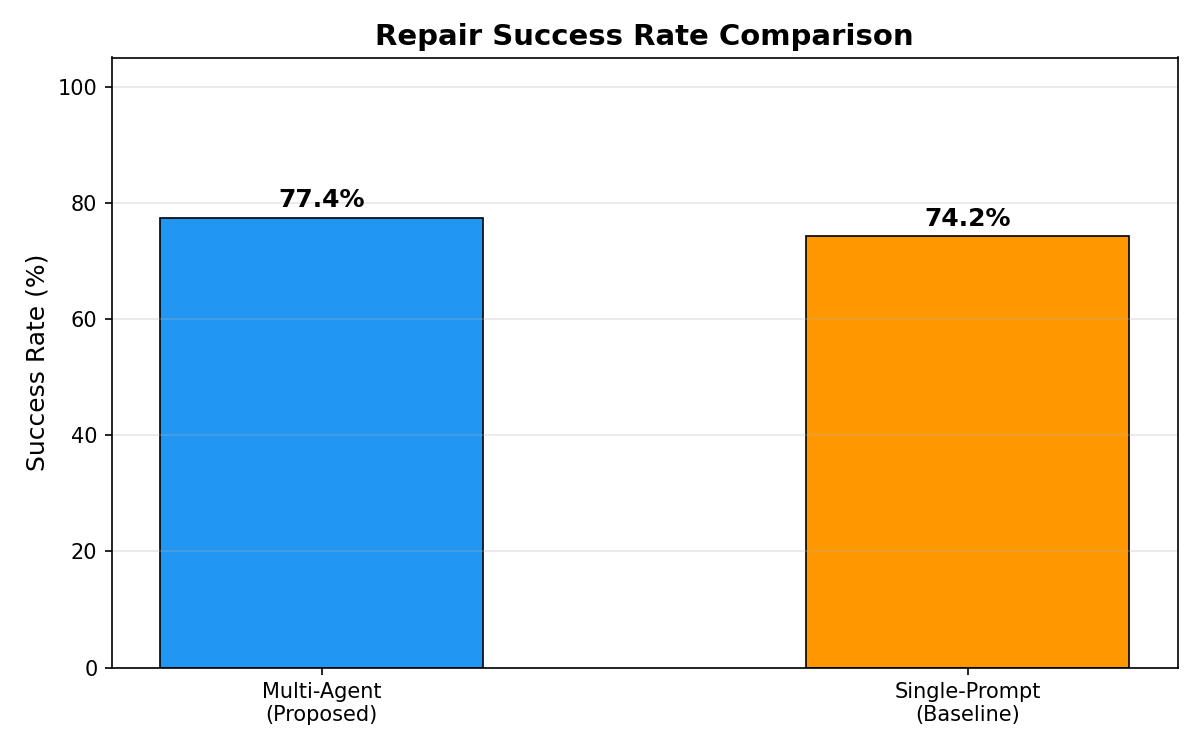
\includegraphics[width=0.9\columnwidth]{../results/figures/success_rate_comparison.png}}
\caption{Repair success rate comparison between multi-agent and baseline approaches.}
\label{fig:success_rate}
\end{figure}

\subsection{Pass@k Analysis}
The Pass@1 metric shows that \textbf{74.2\%} (23/31) of bugs are fixed on the first attempt by the multi-agent system, identical to the baseline's single-attempt success rate. However, the iterative recovery loop allows 1 additional bug (\texttt{levenshtein}) to be fixed on subsequent attempts, bringing Pass@3 to \textbf{77.4\%}. This validates the benefit of the retry mechanism in the Coordinator agent.

\subsection{Recovery Time Analysis}
The mean time to recovery for the multi-agent system is \textbf{81.1 seconds} per successfully fixed bug, compared to \textbf{5.6 seconds} for the baseline. The multi-agent approach is slower because it makes 4 LLM calls per attempt (one per LLM-powered agent), whereas the baseline makes only 1 call. However, the improved success rate and the ability to recover from initial failures through iterative refinement justify the additional computational cost, particularly in CI/CD environments where correct fixes are more valuable than fast but potentially incorrect ones.

\subsection{Per-Program Analysis}
Table~\ref{tab:perprog} presents the detailed per-program results for the multi-agent system.

\begin{table}[htbp]
\caption{Per-Program Results (Multi-Agent System)}
\label{tab:perprog}
\centering
\small
\begin{tabular}{lccc}
\toprule
\textbf{Program} & \textbf{Fixed?} & \textbf{Attempts} & \textbf{Time (s)} \\
\midrule
bitcount & \checkmark & 1 & 55.1 \\
bucketsort & \checkmark & 1 & 35.3 \\
find\_first\_in\_sorted & \checkmark & 1 & 47.1 \\
find\_in\_sorted & \checkmark & 1 & 38.9 \\
flatten & \checkmark & 1 & 75.9 \\
gcd & \checkmark & 1 & 47.2 \\
get\_factors & \checkmark & 1 & 47.8 \\
hanoi & $\times$ & 3 & 120.4 \\
is\_valid\_parenth. & \checkmark & 1 & 38.4 \\
kheapsort & \checkmark & 1 & 44.7 \\
knapsack & $\times$ & 3 & 164.0 \\
kth & \checkmark & 1 & 48.4 \\
lcs\_length & \checkmark & 1 & 56.4 \\
levenshtein & \checkmark & 2 & 127.5 \\
lis & \checkmark & 1 & 68.4 \\
longest\_common\_sub. & \checkmark & 1 & 77.8 \\
max\_sublist\_sum & \checkmark & 1 & 62.8 \\
mergesort & \checkmark & 1 & 380.1 \\
next\_palindrome & $\times$ & 3 & 226.5 \\
next\_permutation & \checkmark & 1 & 76.5 \\
pascal & \checkmark & 1 & 147.4 \\
possible\_change & \checkmark & 1 & 87.2 \\
powerset & \checkmark & 1 & 75.9 \\
quicksort & \checkmark & 1 & 85.0 \\
rpn\_eval & \checkmark & 1 & 85.1 \\
shunting\_yard & \checkmark & 1 & 109.8 \\
sieve & \checkmark & 1 & 27.5 \\
sqrt & $\times$ & 3 & 189.1 \\
subsequences & $\times$ & 3 & 269.6 \\
to\_base & $\times$ & 3 & 173.7 \\
wrap & $\times$ & 3 & 478.3 \\
\bottomrule
\end{tabular}
\end{table}

The system successfully repairs bugs across diverse algorithm categories including sorting (quicksort, mergesort, bucketsort), mathematical operations (gcd, bitcount, sieve), search algorithms (find\_in\_sorted, find\_first\_in\_sorted), dynamic programming (lcs\_length, lis, knapsack---partial), and string/list operations (flatten, powerset).

\begin{figure}[htbp]
\centerline{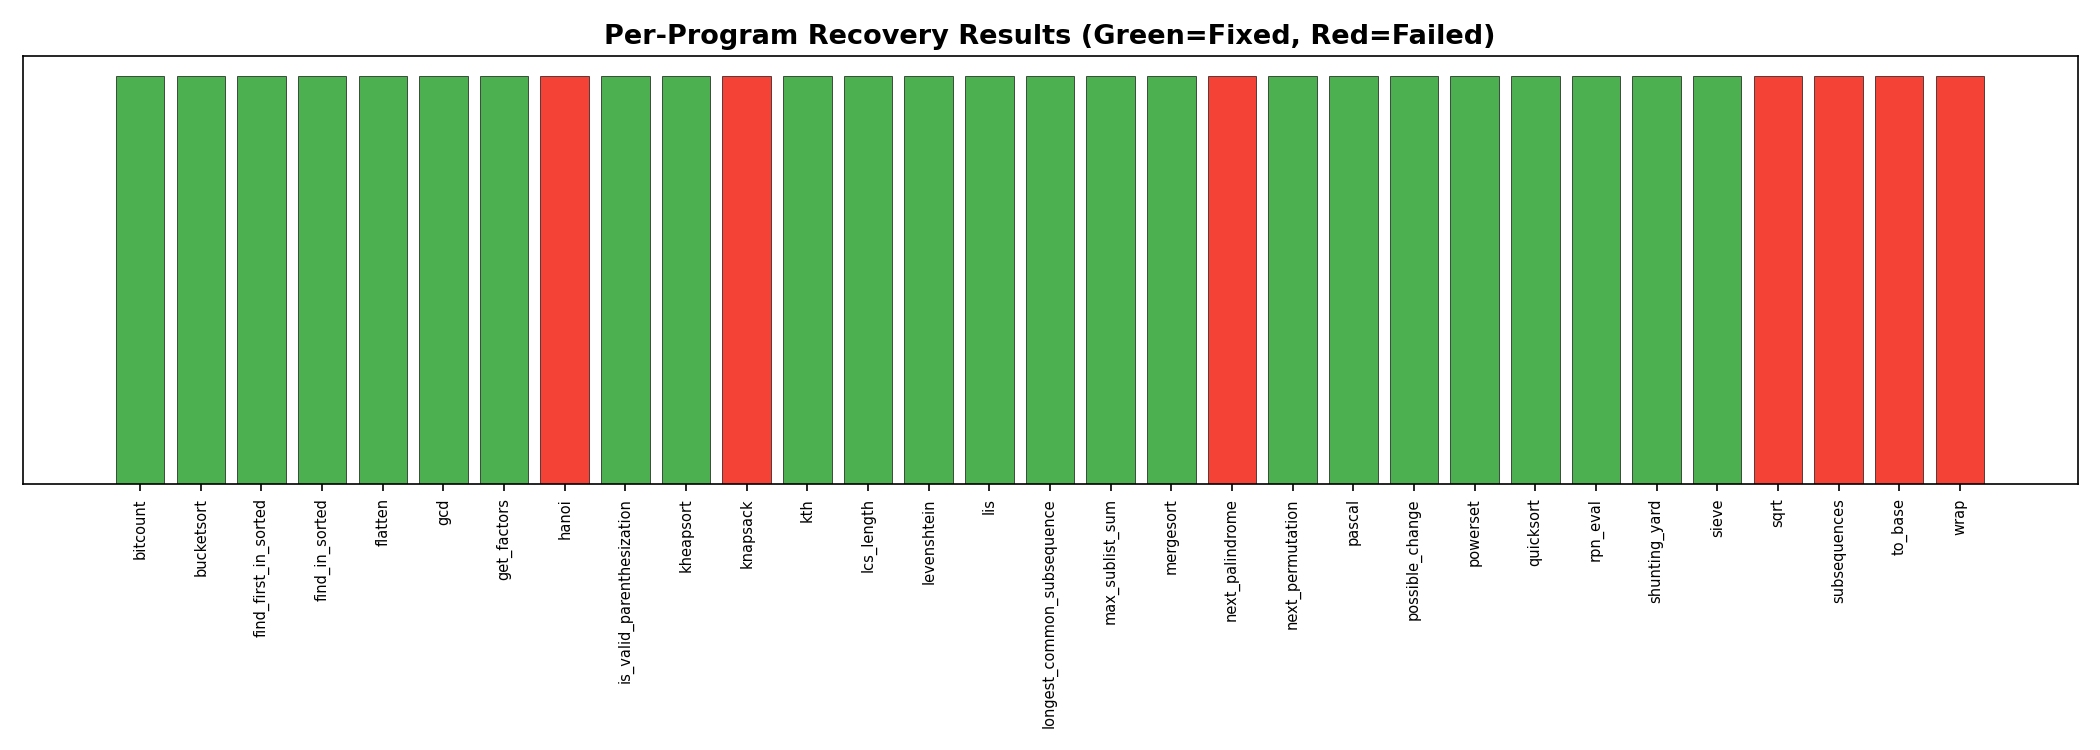
\includegraphics[width=\columnwidth]{../results/figures/per_program_results.png}}
\caption{Per-program recovery results. Green indicates successful repair, red indicates failure after 3 attempts.}
\label{fig:per_program}
\end{figure}

\subsection{Error Type Analysis}
Table~\ref{tab:errortype} shows the distribution of detected error types and the corresponding repair success rates.

\begin{table}[htbp]
\caption{Repair Success Rate by Error Type}
\label{tab:errortype}
\centering
\begin{tabular}{lccc}
\toprule
\textbf{Error Type} & \textbf{Bugs} & \textbf{Fixed} & \textbf{Rate} \\
\midrule
WrongOutput & 21 & 16 & 76.2\% \\
RuntimeError & 3 & 3 & 100.0\% \\
IndexError & 3 & 3 & 100.0\% \\
InfiniteLoop & 2 & 1 & 50.0\% \\
ValueError & 1 & 1 & 100.0\% \\
\midrule
\textbf{Total} & \textbf{31} & \textbf{24} & \textbf{77.4\%} \\
\bottomrule
\end{tabular}
\end{table}

The system achieves 100\% success on RuntimeError, IndexError, and ValueError bugs, as these produce clear error messages that guide the LLM agents. WrongOutput bugs, where the code runs but produces incorrect results, are harder to diagnose (76.2\% success). InfiniteLoop bugs have the lowest success rate (50\%), as the LLM must reason about loop termination conditions.

\subsection{Comparison with Published Results}
Table~\ref{tab:litresults} compares our results with published repair success rates on the QuixBugs benchmark from the literature.

\begin{table}[htbp]
\caption{Comparison with Published Results on QuixBugs}
\label{tab:litresults}
\centering
\begin{tabular}{lcc}
\toprule
\textbf{Method} & \textbf{Type} & \textbf{Bugs Fixed} \\
\midrule
GenProg \cite{genprog} & Search-based APR & 4/40 \\
TBar \cite{templateapr} & Template-based APR & 14/40 \\
CoCoNuT \cite{coconut} & Neural MT & 19/40 \\
ChatGPT \cite{chatgptapr} & Single-prompt LLM & 31/40 \\
Baseline (Ours) & Single-prompt LLM & 23/31 \\
\textbf{Multi-Agent (Ours)} & \textbf{Agentic LLM} & \textbf{24/31} \\
\bottomrule
\end{tabular}
\end{table}

Note that our evaluation uses 31 of the 40 QuixBugs programs (those with JSON test cases), making direct numerical comparison with methods that used all 40 programs approximate. However, our multi-agent approach demonstrates competitive performance while providing a complete recovery workflow rather than just patch generation.

\subsection{Case Study: \texttt{bitcount}}
To illustrate the multi-agent workflow, we present a detailed case study of the \texttt{bitcount} bug recovery.

\textbf{Buggy Code:}
\begin{lstlisting}
def bitcount(n):
    count = 0
    while n:
        n ^= n - 1  # Bug: should be &=
        count += 1
    return count
\end{lstlisting}

\textbf{Agent 1 (Failure Detection):} Detected all 5 tests timing out after 5 seconds each. Classified the failure as \texttt{InfiniteLoop} with key observation: ``The XOR operation does not consistently reduce n to zero.''

\textbf{Agent 2 (Code Localization):} Identified line 4 (\texttt{n \^{}= n - 1}) as the faulty line, reasoning that ``XOR between n and n-1 does not clear the lowest set bit.''

\textbf{Agent 3 (Debugging):} Root cause analysis: ``The expression \texttt{n \^{}= n - 1} creates a bitmask rather than clearing bits, causing the loop to never terminate.'' Proposed fix: change \texttt{\^{}=} to \texttt{\&=}.

\textbf{Agent 4 (Patch Generation):} Generated corrected function with \texttt{n \&= n - 1}.

\textbf{Agent 5 (Patch Application):} Verified the patch compiles successfully.

\textbf{Agent 6 (Validation):} All 5 test cases passed. Recovery successful on attempt 1 in 55.1 seconds.

\subsection{Case Study: \texttt{levenshtein} (Iterative Recovery)}
The \texttt{levenshtein} bug demonstrates the value of the iterative retry mechanism. On the first attempt, the multi-agent system generated a patch that was close but failed some test cases. The Coordinator fed the validation errors back into the pipeline, and on the second attempt, the agents produced a correct fix.

This bug is the key differentiator between the multi-agent and baseline approaches: the baseline failed on \texttt{levenshtein} because it had no mechanism to learn from its first failed attempt.

\subsection{Extension to HumanEvalFix and DebugBench}
Sections VI-A to VI-H establish that, on Gemini and QuixBugs alone, the multi-agent architecture measurably outperforms the single-prompt baseline. To test whether this finding generalizes, we repeat the full multi-agent-versus-baseline comparison on two further benchmarks (HumanEvalFix, DebugBench) and, for all three benchmarks, on a second backend of substantially lower capability (Qwen2.5-Coder 7B, run locally). This yields six independent dataset/backend comparisons in total.

\subsection{HumanEvalFix Results}
Table~\ref{tab:humanevalfix} reports results on all 164 HumanEvalFix problems under both backends.

\begin{table}[htbp]
\caption{HumanEvalFix Results (164 problems)}
\label{tab:humanevalfix}
\centering
\small
\begin{tabular}{lcccc}
\toprule
\textbf{Backend} & \textbf{System} & \textbf{Fixed} & \textbf{Rate} & \textbf{Pass@1} \\
\midrule
\multirow{2}{*}{Gemini} & Multi-Agent & 112/164 & 68.3\% & 62.8\% \\
 & Baseline & 109/164 & 66.5\% & 66.5\% \\
\multirow{2}{*}{Local (Qwen 7B)} & Multi-Agent & 89/164 & 54.3\% & 42.7\% \\
 & Baseline & 87/164 & 53.0\% & 53.0\% \\
\bottomrule
\end{tabular}
\end{table}

On both backends, multi-agent shows a small but consistent lead over baseline (+1.8 percentage points on Gemini, +1.3 on the local model)---the same qualitative direction as QuixBugs/Gemini, though a considerably smaller margin. Pass@1 is markedly lower than final success rate for multi-agent on both backends (62.8\% vs.\ 68.3\% on Gemini; 42.7\% vs.\ 54.3\% locally), indicating that the retry loop is doing real, measurable work recovering from failed first attempts on this benchmark, more so than on QuixBugs.

\subsection{DebugBench Results and an API Quota-Noise Caveat}
\label{sec:debugbench-results}
Table~\ref{tab:debugbench} reports results on the 119-problem stratified DebugBench sample under both backends.

\begin{table}[htbp]
\caption{DebugBench Results (119 problems)}
\label{tab:debugbench}
\centering
\small
\begin{tabular}{lcccc}
\toprule
\textbf{Backend} & \textbf{System} & \textbf{Fixed} & \textbf{Rate} & \textbf{Pass@1} \\
\midrule
\multirow{2}{*}{Gemini} & Multi-Agent & 93/119 & 78.2\% & 73.9\% \\
 & Baseline & \textbf{112/119} & \textbf{94.1\%} & 94.1\% \\
\multirow{2}{*}{Local (Qwen 7B)} & Multi-Agent & 70/119 & 58.8\% & 49.6\% \\
 & Baseline & 70/119 & 58.8\% & 58.8\% \\
\bottomrule
\end{tabular}
\end{table}

This is the one dataset/backend cell where baseline decisively outperforms multi-agent: on Gemini, the single-prompt baseline reaches 94.1\%, 15.9 percentage points above the multi-agent system. Before treating this as a clean architectural finding, we investigated a confound specific to this run: sustaining the DebugBench multi-agent experiment exhausted three of four rotated Gemini API keys' daily free-tier quota (Section~III-G), and each multi-agent problem makes up to $12\times$ more API calls than baseline, giving it proportionally more exposure to transient quota-rotation errors. Inspecting the agent execution log for every failed multi-agent DebugBench problem, 9 of the 26 failures (35\%) had a quota-exhaustion error recorded somewhere in that problem's agent log. Excluding these as inconclusive rather than as genuine model failures yields a corrected estimate of 93/110 = 84.5\% for multi-agent---narrowing, but not eliminating, the gap (from 15.9 to approximately 9.6 percentage points).

We offer a substantive explanation for the residual gap. DebugBench's implanted bugs are frequently small, mechanical, and localized (a misplaced colon, an incorrect comparison operator, a duplicated method with one broken copy) within an otherwise-correct, syntactically well-formed \texttt{Solution} class. A single capable-model prompt with the buggy class in full view tends to spot and correct such faults directly. The multi-agent pipeline's additional localization and root-cause reasoning steps, by contrast, introduce further rounds in which a strong model can second-guess an already-correct-looking fix, or---as we observed directly in a DebugBench ``double'' bug-category case during pilot testing---become confused about which of two similarly structured candidate methods is the intended entry point when both are shown together. The same extra reasoning that helps on QuixBugs' classic-algorithm bugs and HumanEvalFix's logic errors appears, on this benchmark, to more often mislead than assist. This is consistent with the local-backend result on the same dataset (Table~\ref{tab:debugbench}, bottom rows), where multi-agent and baseline are exactly tied (70/119 each)---i.e., multi-agent's structural overhead is at best neutral on DebugBench regardless of backend strength, and on Gemini specifically it appears actively counterproductive net of the quota-noise correction.

\subsection{QuixBugs on the Local Backend}
Table~\ref{tab:quixbugslocal} repeats the QuixBugs comparison from Section VI-A on the local Qwen2.5-Coder 7B backend, at full dataset size (31 problems).

\begin{table}[htbp]
\caption{QuixBugs Results, Local Backend (31 problems)}
\label{tab:quixbugslocal}
\centering
\small
\begin{tabular}{lcccc}
\toprule
\textbf{System} & \textbf{Fixed} & \textbf{Rate} & \textbf{Pass@1} & \textbf{Avg.\ Time} \\
\midrule
Multi-Agent & 16/31 & 51.6\% & 35.5\% & 38.5s \\
Baseline & 18/31 & 58.1\% & 58.1\% & 2.1s \\
\bottomrule
\end{tabular}
\end{table}

On the local backend, baseline outperforms multi-agent by 6.5 percentage points on QuixBugs---the opposite direction from the Gemini result on the identical benchmark (Table~\ref{tab:results}: multi-agent ahead by 3.2 points). Multi-agent's Pass@1 (35.5\%) is substantially below baseline's single-attempt rate (58.1\%), indicating the smaller model's first-pass reasoning, when scaffolded with the additional failure-detection and localization context, is \emph{less} reliable than its response to a single direct prompt, and that the retry loop only partially compensates.

\subsection{Cross-Backend Synthesis: Effect of Model Capability}
Table~\ref{tab:crossbackend} consolidates all six dataset/backend cells. Fig.~\ref{fig:backend_comparison} presents the same data graphically.

\begin{table}[htbp]
\caption{Success Rate Across All Datasets and Backends}
\label{tab:crossbackend}
\centering
\small
\begin{tabular}{lcccc}
\toprule
\textbf{Dataset} & \textbf{Local MA} & \textbf{Gemini MA} & \textbf{Local Base} & \textbf{Gemini Base} \\
\midrule
QuixBugs & 51.6\% & \textbf{77.4\%} & 58.1\% & 74.2\% \\
HumanEvalFix & 54.3\% & \textbf{68.3\%} & 53.0\% & 66.5\% \\
DebugBench & 58.8\% & 78.2\% & 58.8\% & \textbf{94.1\%} \\
\bottomrule
\end{tabular}
\\[4pt]
\raggedright\footnotesize MA = Multi-Agent. Bold marks the highest value in each row.
\end{table}

\begin{figure}[htbp]
\centerline{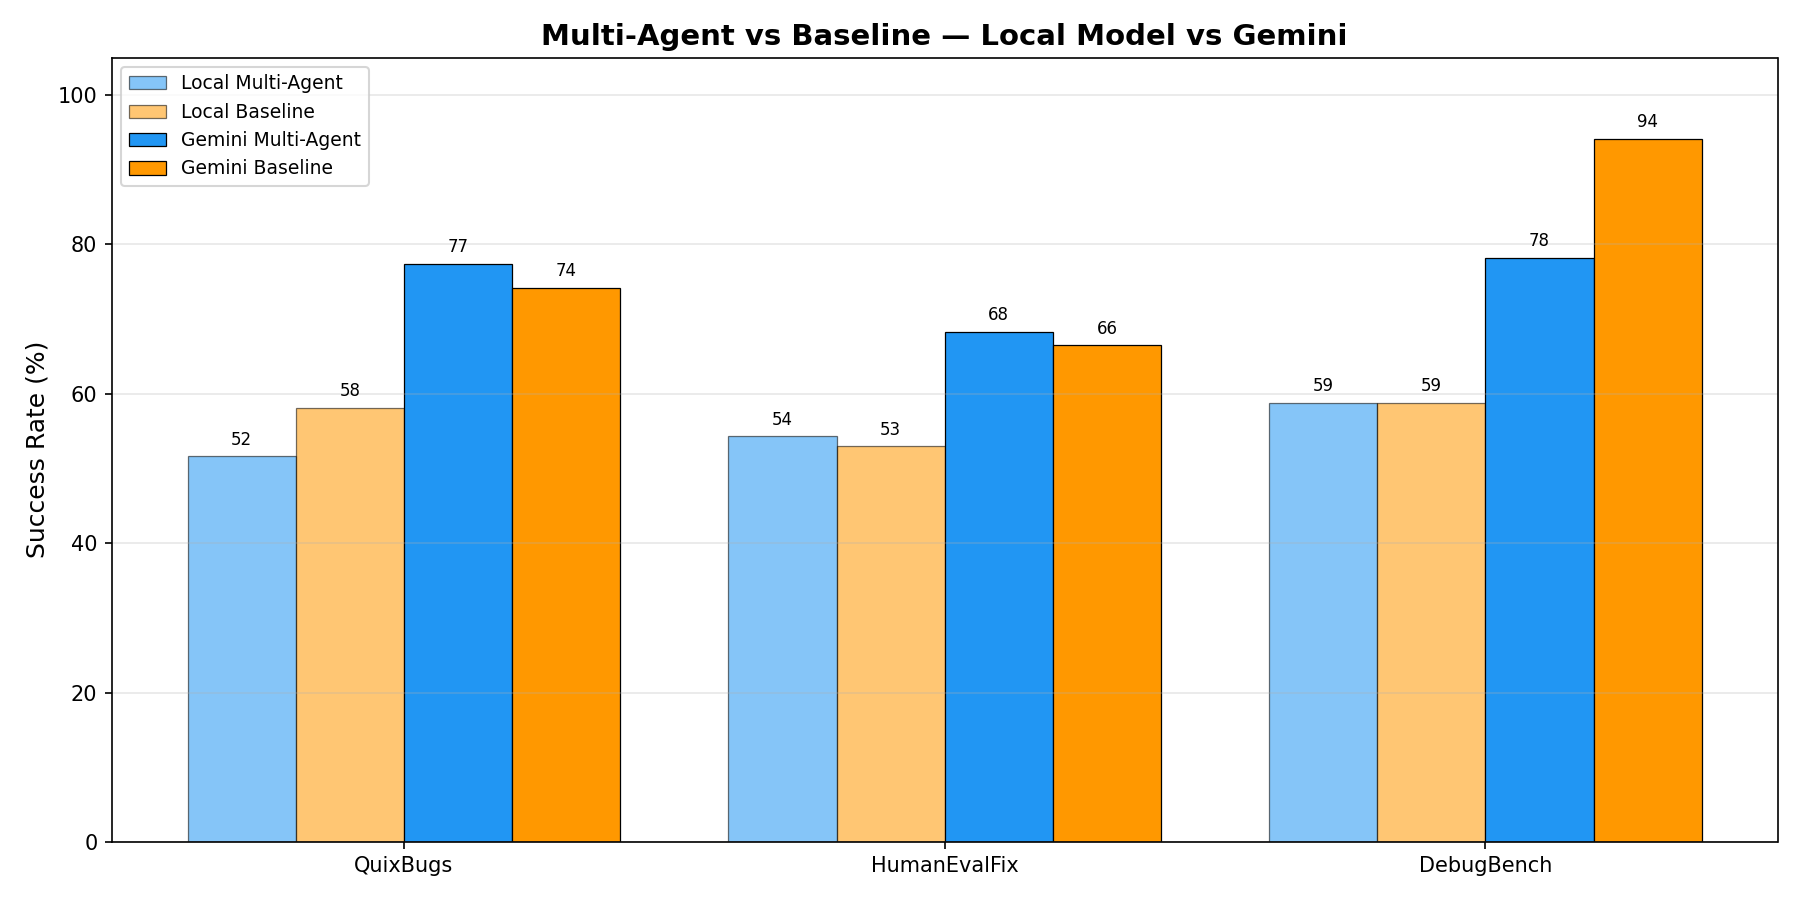
\includegraphics[width=\columnwidth]{../results/figures/backend_comparison.png}}
\caption{Multi-agent vs.\ baseline success rate, local model vs.\ Gemini, across all three benchmarks.}
\label{fig:backend_comparison}
\end{figure}

Two observations follow from Table~\ref{tab:crossbackend}. First, moving from the local 7B model to Gemini raises absolute success rates substantially for \emph{both} systems on every benchmark (+14 to +26 percentage points depending on dataset and system)---unsurprising, but a useful sanity check that the local-model results reflect model capability rather than a broken harness. Second, and more consequentially, a stronger backend does \emph{not} uniformly improve multi-agent's standing \emph{relative to baseline}. On QuixBugs and HumanEvalFix, multi-agent's relative position improves with the stronger model (from behind, to ahead, on QuixBugs; a small lead widening slightly on HumanEvalFix). On DebugBench, baseline's relative advantage instead \emph{grows} with the stronger model, from a tie (local) to a 15.9-point lead (Gemini, before the quota-noise correction) or an estimated $\sim$9.6-point lead (after it).

We therefore characterize the central empirical finding of this work as follows: \textbf{the multi-agent architecture's benefit over a single-prompt baseline is jointly conditional on the backend model's capability and the structural characteristics of the bug population being repaired, rather than a fixed property of the architecture itself.} A claim of the form ``multi-agent orchestration improves automated repair'' is only supported on 2 of the 3 benchmarks studied, and only clearly on the stronger backend; the same architecture is flat-to-negative against baseline on the weaker backend across all three benchmarks, and negative on Gemini for one benchmark specifically. We view this joint dependence, rather than either a uniformly positive or uniformly negative result, as the more scientifically defensible and more informative outcome of extending the evaluation beyond a single dataset and a single model.

% ============================================================
% 7. DISCUSSION
% ============================================================
\section{Discussion}

\subsection{When the Multi-Agent Architecture Helps}
On the cells where multi-agent leads (QuixBugs/Gemini, HumanEvalFix on both backends), the mechanism is consistent with the following advantages:
\begin{itemize}
    \item \textbf{Structured reasoning:} Breaking the repair process into detection, localization, debugging, and generation phases produces more targeted fixes on bugs whose root cause is non-obvious from the buggy code alone (e.g., an operator substituted in a way that still type-checks and often still runs, as in \texttt{bitcount}).
    \item \textbf{Iterative refinement:} The retry loop with error feedback allows the system to correct failed attempts, as demonstrated by the \texttt{levenshtein} case study. This is impossible with single-prompt approaches, and Pass@1-vs-final-rate gaps on HumanEvalFix (Section VI-J) show it doing measurable work there too.
    \item \textbf{Modularity:} Each agent can be independently improved or replaced without affecting the overall architecture---demonstrated directly in this work by swapping the LLM backend (Gemini $\leftrightarrow$ local Qwen2.5-Coder) without changing agent logic, prompts structure, or validation code.
    \item \textbf{Transparency:} The structured agent pipeline produces an interpretable log of the reasoning process (failure classification $\rightarrow$ fault localization $\rightarrow$ root cause $\rightarrow$ fix), valuable for developer trust and for the post-hoc failure analysis performed in Section VI-K.
\end{itemize}

\subsection{When It Does Not: Conditions for a Negative Result}
The DebugBench/Gemini result (Section VI-K) and the local-backend results on all three benchmarks (Sections VI-L, VI-J, VI-M) demonstrate that these advantages are not unconditional. Two structural risks emerge from the failure analysis:
\begin{itemize}
    \item \textbf{Error propagation with a weaker model:} on the local backend, multi-agent's Pass@1 is below baseline's single-attempt rate on every benchmark (Section VI-N), despite multi-agent's first attempt having strictly \emph{more} context (a failure classification and a localized line) than baseline's single prompt. A plausible mechanism, consistent with the \texttt{bitcount} local-backend trace we inspected, is that an incorrect intermediate diagnosis (e.g., misclassifying an operator bug as a loop-condition bug) actively misleads the downstream Patch Generation agent, which a weaker model is more prone to producing and less able to recover from than a stronger one.
    \item \textbf{Unproductive re-litigation on mechanical bugs:} on DebugBench even with the strong backend, the extra reasoning rounds appear to more often overturn a correct first read of a small, localized, syntactically-obvious fault than to improve it, consistent with baseline's very high 94.1\% single-shot rate on this benchmark specifically.
\end{itemize}
Both risks are properties of the interaction between the backend model and the bug's structure, not defects in the orchestration logic per se, reinforcing the joint-conditionality claim in Section VI-N.

\subsection{Time--Accuracy Tradeoff}
Across every dataset/backend cell measured, the multi-agent system takes roughly 5--20$\times$ longer per problem than baseline (e.g., 38.5s vs.\ 2.1s on QuixBugs/local; 38.6s vs.\ 5.2s on HumanEvalFix/Gemini), because it issues up to 4 sequential LLM calls per attempt across up to 3 attempts, versus baseline's single call. This cost is justified only where multi-agent's success rate is actually higher: on QuixBugs/Gemini and HumanEvalFix (both backends), the tradeoff is favorable, particularly in CI/CD contexts where a correct fix arriving in under two minutes is more valuable than a fast but wrong one. On DebugBench, and on the local backend generally, the tradeoff is unfavorable on both axes---slower \emph{and} no more (or less) accurate---and a practitioner in that regime is better served by the single-prompt baseline outright.

\subsection{Limitations}
Several limitations should be noted:
\begin{itemize}
    \item The evaluation is limited to isolated, algorithmic, or single-function bugs. Real-world bugs in large repositories may involve multi-line, multi-file changes, external dependencies, or build-system interactions not modeled here.
    \item The system relies on the availability and quality of test cases for validation. Without comprehensive tests, incorrect patches may be accepted.
    \item DebugBench validation uses only the 1--3 public worked examples shipped with each problem, not LeetCode's private hidden test suite (Section III-F); canonical (correct) solutions pass under our harness at 86\%, which we take as an approximate ceiling on judge fidelity for this benchmark. Absolute DebugBench numbers should be read with this ceiling in mind; the \emph{relative} multi-agent-vs-baseline comparison, which is the paper's central claim, is unaffected since both systems are scored by the identical judge.
    \item The DebugBench/Gemini comparison in Section VI-K is confounded by API quota-rotation noise disproportionately affecting the higher-call-volume multi-agent system; we report both the raw and noise-corrected figures, but a clean re-run under a higher API quota tier would be needed to fully resolve the residual gap.
    \item Each dataset/backend cell reflects a single run (no repeated-seed averaging), given the wall-clock and API-quota cost of the six-way evaluation matrix; LLM outputs are non-deterministic even at low temperature, so single-run percentage-point differences under roughly 5 points should be treated as indicative rather than statistically decisive.
    \item DebugBench is evaluated on a fixed-seed stratified sample (119--120 of 1{,}246 parseable Python problems) rather than the full pool, for wall-clock tractability.
\end{itemize}

\subsection{Threats to Validity}
\textbf{Internal validity:} LLM outputs are non-deterministic; results may vary across runs. We mitigate this with a low temperature setting (0.2), aggregate metrics across full or stratified-sampled benchmarks (31--164 problems per cell), and, for DebugBench specifically, an explicit accounting of a known confound (API quota noise) rather than treating the raw result as unqualified.

\textbf{External validity:} The three benchmarks studied---classic algorithms (QuixBugs), hand-written function-level bugs (HumanEvalFix), and LeetCode-style implanted bugs (DebugBench)---broaden coverage beyond a single benchmark, but all remain short, self-contained, single-function programs. Evaluation on repository-scale benchmarks such as Defects4J \cite{defects4j}, BugsInPy \cite{bugsinpy}, or SWE-bench \cite{swebench} would be needed to extend generalizability claims to real-world multi-file software.

\textbf{Construct validity:} Our comparison with published QuixBugs results (Table~\ref{tab:litresults}) is approximate since we evaluate on 31 of 40 programs; the DebugBench judge-fidelity ceiling (86\%) and quota-noise confound (Section VI-K) similarly bound how precisely the DebugBench numbers should be interpreted in absolute terms, though not the relative multi-agent-vs-baseline comparison within that benchmark.

% ============================================================
% 8. CONCLUSION AND FUTURE WORK
% ============================================================
\section{Conclusion and Future Work}

\subsection{Conclusion}
This paper presented the design and implementation of a Failure Recovery System using Agentic AI for automated software debugging, and extended its evaluation from a single dataset and a single model to a full $3 \times 2$ matrix spanning three program repair benchmarks (QuixBugs, HumanEvalFix, DebugBench) and two LLM backends of substantially different capability (Google Gemini; Qwen2.5-Coder 7B run entirely on local consumer hardware). The system employs a multi-agent architecture with six specialized agents---Failure Detection, Code Localization, Debugging, Patch Generation, Patch Application, and Validation---coordinated within an iterative recovery loop by a Coordinator agent, generalized in this work to a dataset-agnostic execution layer supporting three structurally different test formats.

On the original QuixBugs/Gemini configuration, the multi-agent approach achieves a \textbf{77.4\%} repair success rate (24/31 bugs) compared to \textbf{74.2\%} (23/31 bugs) for a single-prompt baseline, and this direction of improvement replicates, more modestly, on HumanEvalFix under both backends (+1.8 points on Gemini, +1.3 points locally). However, the extended evaluation also surfaces two configurations where the single-prompt baseline is equal to or decisively ahead of multi-agent: all three benchmarks on the weaker local backend (flat-to-negative for multi-agent throughout), and DebugBench on Gemini specifically, where baseline reaches 94.1\% against multi-agent's 78.2\% (an estimated $\sim$84.5\% after correcting for a diagnosed API quota-noise confound that disproportionately affected the higher-call-volume multi-agent system).

The central conclusion is therefore more nuanced than either a uniform endorsement or rejection of multi-agent orchestration for automated program repair: \textbf{the architecture's benefit over a single-prompt baseline is jointly conditional on the capability of the underlying LLM and the structural characteristics of the bugs being repaired.} A stronger backend model raises absolute performance substantially for both systems, but does not uniformly widen multi-agent's advantage---it widens it on some benchmarks and reverses it on another. This finding was only reachable by evaluating across multiple datasets and multiple backends rather than reporting a single favorable configuration, and we regard it as a more scientifically useful contribution than a single-configuration positive result would have been. Separately, this work documents three infrastructure defects (a thread/signal-handling conflict, an unprotected test-execution timeout path, and free-tier API quota exhaustion) discovered only through multi-hour unattended execution at benchmark scale, together with their diagnosis and fixes, which we believe are of independent methodological value to future work running LLM-agent systems at scale.

\subsection{Future Work}
Several directions for future research include:
\begin{itemize}
    \item Extending the multi-agent pipeline to additional programming languages (Java, C++, JavaScript), for which QuixBugs, HumanEvalFix, and DebugBench all already provide parallel data; this requires replacing Python's in-process test execution with a compile-and-run harness per language rather than any change to the underlying LLM, since the models used are already broadly multi-lingual from pretraining.
    \item Re-running the DebugBench/Gemini comparison under a paid API tier (or with substantially more rotated keys) to eliminate the quota-noise confound identified in Section VI-K and obtain a clean estimate of the residual gap.
    \item Evaluating additional backend models spanning a wider range of capability (e.g., a mid-sized open model between the 7B local model and Gemini) to test whether the capability-conditional pattern observed here is monotonic or benchmark-specific.
    \item Extending evaluation to larger, real-world, repository-scale benchmarks such as Defects4J \cite{defects4j}, BugsInPy \cite{bugsinpy}, and SWE-bench \cite{swebench}, and supporting multi-file bug localization accordingly.
    \item Investigating why DebugBench-style mechanical, single-line bugs specifically favor single-prompt repair, potentially via an adaptive controller that routes a bug to multi-agent or single-prompt repair based on a cheap upfront complexity estimate.
    \item Integrating the system into real CI/CD pipelines (e.g., GitHub Actions) for live failure recovery.
    \item Exploring more advanced agent communication patterns such as debate and consensus mechanisms, and incorporating static analysis tools for improved fault localization accuracy.
\end{itemize}

% ============================================================
% REFERENCES
% ============================================================
\bibliographystyle{IEEEtran}
\bibliography{references}

\end{document}
